\documentclass[a4paper,10pt]{article}
\usepackage[utf8]{inputenc}
\usepackage{amsmath}
\usepackage{braket}
\usepackage{todonotes}
\usepackage{listings}
\usepackage{graphicx}
\usepackage[mathscr]{euscript}
\usepackage{float}
% \usepackage[capposition=top, font=small]{floatrow}
\usepackage{hyperref}
%\hypersetup{
%    colorlinks=true,
%   linkcolor=blue,
%    filecolor=magenta,      
%    urlcolor=blue,}
 
\urlstyle{same}

%opening
\title{Thermalisation of Ultracold Bose Gases on Optical Lattices}
\author{Nikolas M. Mitchell}


\begin{document}

\maketitle

\begin{abstract}

Systems of ultra-cold gases in light-induced periodic potentials (optical lattices) are of great experimental and theoretical interest, and have been since the first experimental 
realisation of Bose-Einstein condensation in 1995. \todo{I think I should include some ``flavour'' here with vaguely interesting general statements about thermodynamics}
This is largely due to the parallels between the behaviour of BECs in an optical lattice and condensed matter systems, where 
electrons can be modelled as moving on a lattice generated by the periodic array of atom cores \cite{Bloch2012}. This project 
investigates the time evolution of a system of bosons prepared in a far-from-equilibrium state on a one-dimensional or two-dimensional
optical lattice. The main focus is on determining how the tunneling energies and the strength of the interparticle interactions influence
whether or not the system exhibits relaxation to a thermal state. For systems in which revival to the initial state occurs regularly (those which don't thermalise), 
a method for calculating the revival period is developed. For the systems which exhibit thermalisation, we attempt to characterise the long term
states using [ETH, entropy of entanglement, whatever I actually end up doing].



\end{abstract}
\newpage
\section{Experimental advantages of working with bosons on optical lattices}
 
\begin{figure}[H]
 \begin{center}
   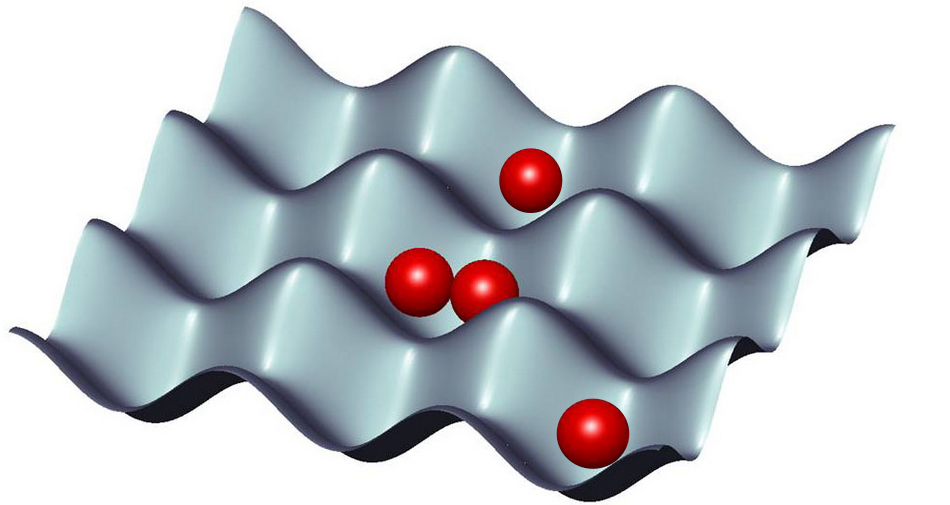
\includegraphics[width=8cm]{bosons_on_lattice}
 \end{center}
 \caption{Bosons on a 2D optical lattice.}
 \end{figure}
\todo{I got the image that this picture is based on from https://www.uibk.ac.at/th-physik/qo/research/opticallattices.html.en . How do I reference that properly?}


In a typical condensed matter system, we can model electrons as moving on a lattice potential produced by a periodic array of atom cores. 
We can simulate this type of system with ultracold atoms using optical lattices to generate the periodic potential. An optical lattice is 
produced by overlapping multiple laser beams and making use of the interference pattern. The alternating bright and dark areas of the interference
pattern act as a periodic potential on the atoms through the optical dipole force \cite{Bloch2012}. By superimposing different combinations of laser
beams at particular frequencies and amplitudes, any lattice geometry that can be constructed via Fourier synthesis can, in principle, be produced \cite{Bloch2012}.
This fine degree of control over the lattice parameters, in conjunction with the ability to tune the strength of interparticle interactions by 
manipulating Feshbach resonances \cite{Chin2010}, makes ultracold bosons on optical lattices an excellent arena in which to explore various model 
Hamiltonians for condensed matter systems and quantum optics. \\\\

There are further advantages which can make conducting experiments with ultracold bosons on optical lattices more attractive than working with 
solids directly. One is that there are always impurities present in the solids we find in nature. These impurities can have significant impacts
on the properties of the solid which cannot necessarily be accounted for by a perturbative approach which assumes these effects 
to be small. \todo{reference this at some point from the book I meant to get from David}\\\\

\todo{see square brackets} [Here I can either say a) or b).\\ a) Optical lattices are highly uniform, so when dealing with bosons on optical lattices this problem of impurities does not arise.\\
b) Is this statement from \cite{Bloch2012} relevant to this question?
\begin{figure}[H]
 \begin{center}
   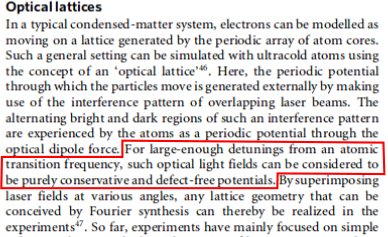
\includegraphics[width=8cm]{optical_lattices_Bloch}
 \end{center}
 \end{figure}
]
Another benefit of working with bosons on optical lattices is that we can easily control the state of each of the particles on the lattice. Furthermore, 
the potential can be altered or switched off entirely during the experiment, which is a feature that is not available in any solid state experiment \cite{Morsch2006}.



\section{First quantised representation}
This paper will deal exclusively with bosons on optical lattices, and not investigate cases involving fermions.
There are a number of different contributions to the Hamiltonian for bosons on optical lattices, and these contributions can be seen to have analogues in condensed matter systems.
The individual bosons will have kinetic energy, and the potential created by the lattice also contributes to how the system evolves in time, so it must feature in the Hamiltonian.
The bosons may be interacting (we will assume this only occurs if they occupy the same lattice sites), and there may also be an external potential imposed that can vary in strength
from site to site. From this reasoning, we can construct a first quantised Hamiltonian for a 1D system of interacting bosons on an optical lattice, in the presence of an external potential $V_{\text{ext}}$
\begin{equation}
  \label{eq:HamiltonianCoordinateRepresentation}
 \hat{H}=\sum_{i}-\frac{\hbar^{2}}{2m}  \partial_{x_{i}}^2+\sum_{i}V_{\text{lattice}}(R_{i})+V_{\text{ext}}(x)+\frac{U}{2}\sum_{i,j}\delta(x_{i}-x_{j}).
\end{equation}

Similar Hamiltonians are frequently used to describe systems of electrons on atomic lattices.
\\\\


\section{Many-particle wavefunctions and identical particles}
The Hamiltonian in the previous section would act on a bosonic many-particle wavefunction. A single particle wavefunction $\psi{\vec{r}}$ is 
defined within a Hilbert space $\mathcal{H}$, which is the space of complex, square integrable functions. It must satisfy $\int d^3\vec{r}|\psi(\vec{r})|^2<\infty$.
A wavefunction that represents the state of $N$ indistinguishable particles, $\psi(\vec{r}_{1},\vec{r}_{2},\dots,\vec{r}_{N})$ is defined within $\mathcal{H}^N$, where
$\mathcal{H}^N$ is constructed as the tensor product $N$ single-particle Hilbert spaces:
\begin{equation}
 \mathcal{H}^N=\mathcal{H}\otimes \mathcal{H} \otimes \dots\otimes \mathcal{H}.
\end{equation}

The wavefunctions in this space are also subject to normalisation constraints, i.e.,

\begin{equation*}
 \int d^3\vec{r_1} d^3\vec{r_2}\dots d^3\vec{r_N} |\psi(\vec{r}_{1},\vec{r}_{2},\dots,\vec{r}_{N})|^2<\infty.
\end{equation*}

Whilst all functions satisfying the above constraints can be legitimately defined mathematically, only a small subset are found to occur in nature - those which are either 
entirely symmetric or antisymmetric under particle exchange. The set of indistinguishable particles which are entirely symmetric under particle exchange are defined as bosons.
This project will not investigate scenarios involving the particles that display exchange antisymmetry (fermions), so we will be working within the space $S_N\mathcal{H}^N$ . We can formally
express the requirement of exhange symmetry for bosonic systems as \cite{Negele1988}

\begin{equation*}
 \psi({\vec{r}_{\mathcal{P}1},\vec{r}_{\mathcal{P}2},\dots,\vec{r}_{\mathcal{P}N}})= \psi(\vec{r}_{1},\vec{r}_{2},\dots,\vec{r}_{N}),
\end{equation*}
where $\{\mathcal{P}1,\mathcal{P}2,\dots,\mathcal{P}N  \}$ represents any permutation, $\mathcal{P}$, of the set $\{1,2,\dots,N\}$.

Let us first consider the case of two indistinguishable bosons. We have not yet determined the eigenstates 
of our Hamiltonian, but if we suppose we have the set of normalised single-particle wavefunctions $\{\ket{\lambda}\}$, and we have one boson in state $\ket{\lambda_1}$ and another
in state $\ket{\lambda_2}$, then we can write the two-particle wavefunction as

\begin{equation}
 \psi(\vec{r}_{1},\vec{r}_{2})=\frac{1}{\sqrt{2}}\big(\braket{\vec{r}_{1}|\lambda_1}\braket{\vec{r}_{2}|\lambda_2}+\braket{\vec{r}_{1}|\lambda_2}\braket{\vec{r}_{2}|\lambda_1}\big),
\end{equation}
or in Dirac bra-ket notation, the two-body states would be represented as
\begin{equation}
 \ket{\lambda_1,\lambda_2}=\frac{1}{\sqrt{2}}\big(\ket{\lambda_1}\otimes \ket{\lambda_2}+\ket{\lambda_2}\otimes\ket{\lambda_1}\big)
\end{equation}

The number of permutations that one must account for grows extremely quickly as particle number increases. A properly symmetrised and normalised $N$-body state can be
represented as \cite{Altland2010}
\begin{equation}
 \ket{\lambda_1,\lambda_2,\dots,\lambda_N}=\frac{1}{\sqrt{N!\prod_{\lambda=0}^{\infty}{n_{\lambda}}}}
 \sum_{\mathcal{P}}\ket{\lambda_{\mathcal{P}1}}\otimes \ket{\lambda_{\mathcal{P}2}}\otimes\dots\otimes\ket{\lambda_{\mathcal{P}N}}
\end{equation}
where $n_{\lambda}$ is the number of particles in state $\lambda$, and the summation runs over all $N!$ permutations $\mathcal{P}$ of the set of quantum numbers $\{ \lambda_1,\dots,\lambda_N\}$.
\\\\
This formalism has a number of shortcomings. The most important of these for this project is that it is extremely cumbersome for practical computation because of the large number of entities that need to be 
represented. To avoid this, we shall adopt the second quantised formalism, which is much better suited to dealing concisely with large numbers of indistinguishable particles.
\newpage
\section{Second Quantisation}
\subsection{The Occupation Number Representation}
The formalism that we have hitherto discussed explicitly represents a significant amount of redundant information, in the sense that it deals separately with the scenarios ``particle 1 in state $\lambda_1$ and 
particle 2 in state $\lambda_2$'' and ``particle 2 in state $\lambda_1$ and particle 1 in state $\lambda_2$''. Taking into account the indistinguishability of the particles, it is clear that these two scenarios
are identical. A more efficient approach consists of describing the number of particles in a particular state $\lambda_i$, i.e., using the occupation number representation. When doing this, a general 
state can be written as a linear superposition
\begin{equation}
 \ket{\Psi}=\sum_{n_1,n_2,\dots}c_{n_1,n_2,\dots}\ket{n_1,n_2,\dots}.
\end{equation}

In the scenario which this project will be working with, the occupation numbers refer to the number of bosons on a particular site of the lattice.
Having established this, we can define creation and annihilation operators that create and annihilate particles from number eigenstates, that is

\begin{equation}
 \hat{a}_{j}^{\dagger}\ket{n_1,n_2,\dots,n_{j},\dots}=\sqrt{n_j+1}\ket{n_1,n_2,\dots,n_{j}+1,\dots}
\end{equation}
and 

\begin{equation}
 \hat{a}_{j}\ket{n_1,n_2,\dots,n_{j},\dots}=\sqrt{n_j}\ket{n_1,n_2,\dots,n_{j}-1,\dots}.
\end{equation}
These operators have very important commutation relations
\begin{equation}
\begin{align*}
 [\hat{a}_{j}^{\dagger},\hat{a}_{k}^{\dagger}]=0, \ \ \ \ \ [\hat{a}_{j},\hat{a}_{k}]=0,\ \ \ \ [\hat{a}_{j},\hat{a}_{k}^{\dagger}]=\delta_{jk}.
 \end{align*}
\end{equation}
We can also define the number operator $\hat{n}_j=\hat{a}_{j}^{\dagger}\hat{a}_j$ that has the property that
\begin{equation}
 \hat{n}_{j}\ket{n_1,n_2,\dots,n_{j},\dots}=n_{j}\ket{n_1,n_2,\dots,n_{j},\dots}
\end{equation}

The occupation number eigenstates form the basis of the $N$-particle Hilbert space that we are working in (the Fock space $\mathcal{F}^N$), and it 
is useful to observe that any occupation number eigenstate can be created from the empty (or ``vacuum'') state $\ket{0}$ by repeated action of 
creation operators \cite{Altland2010}
\begin{equation}
 \ket{n_1,n_2,\dots}=\prod_i\frac{1}{\sqrt{n_i!}}(\hat{a}_i^{\dagger})^{n_i}\ket{0}
\end{equation}

It may seem that the state space $S_N\mathcal{H}^N$ that we have constructed is not robust enough to accomodate these operators. Indeed, the creation and
annihilation operators take us from the $N$-particle Hilbert space to the $N+1$- and $N-1$-particle Hilbert spaces, respectively. In order to
account for these differences in particle number, we must really be working within the symmetric Fock states $\mathcal{F}_S(\mathcal{H})$, defined by the direct sum \cite{Blank1999}
\begin{equation}
 \mathcal{F}_S(\mathcal{H})=\oplus_{N=0}^\infty S_N\mathcal{H}^N.
\end{equation}

However, we will be working in systems in which the particle number is conserved. Each combination of creation and annihilation operators that appears in the Hamiltonian
will create an equal number of particles to the number destroyed. So for practical purposes we are just working within $S_N\mathcal{H}^N$.

Having established the space and states that we are operating with, we now need to rewrite the Hamiltonian in number state representation, i.e., we need to
``second quantise'' it. 

\subsection{Second Quantisation of the Hamiltonian}
We can second quantise the Hamiltonian initially used to describe our system through the boson field operators, $\hat{\psi}^{\dagger}(x)$ and $\hat{\psi}(x)$, which create and destroy 
particles at particular spatial locations (we will define these more explicitly later). The first two terms in equation \eqref{eq:HamiltonianCoordinateRepresentation} are single-particle
operators for the kinetic and potential energy contributions, and can be transformed to
\begin{equation}
 \int  \hat{\psi}^{\dagger}(x) \bigg(  \sum_{i}-\frac{\hbar^{2}}{2m}  \partial_{x_{i}}^2+\sum_{j}V_{\text{lattice}}(R_{j})  \bigg)    \hat{\psi}(x)dx.
\end{equation}

Bloch's theorem (in 1D) \cite{Bloch1929,Kittel1987} tells us that the eigenstates of a particle in a periodic potential have the form
\begin{equation}
 \phi_q(x)=e^{iqx}u_{q}(x),
\end{equation}
where $q$ is the quasi-momentum and $u_q(x)$ is periodic with the same period as the lattice, $d$. We will be considering scenarios in which the strength of the lattice potential
is such that the bosons are not completely localised, but such that the overlap between the wavefunctions of particles on particular lattice sites have effectively zero overlap 
with non-nearest neighbours. Under these conditions, the wavefunctions can be conveniently described by the localised Wannier functions
\begin{equation}
\psi(R;r)=\frac{1}{d}\int dq\, e^{iRq}\phi_q(x)
\end{equation}
which are superpositions of Bloch functions \cite{Kittel1987,Wannier1937}. This is a useful desciption because the Wannier functions are both orthonormal and, more importantly, complete.
We can use this to rewrite the field operators as 
\begin{equation}
 \hat{\psi}=\sum_j \hat{a}_{j}(t)\psi(R_j-x).
\end{equation}
With this in mind, we can write
\begin{equation}
 \int  \sum_j\hat{a}_j^{\dagger}\psi^{*}(R_j-x) \bigg(  \sum_{i}-\frac{\hbar^{2}}{2m}  \partial_{x_{i}}^2+\sum_{i}V_{\text{lattice}}(R_{i}) 
 \bigg)  \sum_l  \hat{a}_l\psi(R_l-x)dx=\sum_{j,l} J_{j,l}\hat{a}_{j}^{\dagger}\hat{a}_l.
\end{equation}
Here
\begin{equation}
 J_{j,l}=\int  \psi^{*}(R_j-x) \bigg(  \sum_{i}-\frac{\hbar^{2}}{2m}  \partial_{x_{i}}^2+\sum_{i}V_{\text{lattice}}(R_{i}))  \bigg)  \psi(R_l-x)dx
\end{equation}
characterises the strength of the hopping between sites $j$ and $l$, which (intuitively) depends on the combination of the lattice depth and the kinetic energy. We take this hopping strength to be negligible
for sites which are not nearest-neighbours because the localised wavefunctions have exponentially decaying tails, so the overlap is expected to be small. Of the permitted hopping interactions, we assume that each has identical strength. This assumption allows us to write
\begin{equation}
 \int  \hat{\psi}^{\dagger}(x) \bigg(  \sum_{i}-\frac{\hbar^{2}}{2m}  \partial_{x_{i}}^2+\sum_{j}V_{\text{lattice}}(R_{j})  \bigg)    \hat{\psi}(x)dx=J\sum_{i}(\hat{a}^\dagger_{i}\hat{a}_{i+1}+h.c.),
\end{equation}
where $h.c.$ denotes the hermitian conjugate.
We can go through a similar process for the contributions of the external potential and on-site interactions between bosons. The external potential gives an on-site energy that can vary
at different locations in the lattice

\begin{equation}
 \int  \hat{\psi}^{\dagger}(x) V_{\text{ext}}(x)  \hat{\psi}(x)dx = \sum_i \epsilon_i \hat{a}_i^{\dagger}\hat{a}_i.
\end{equation}

The term for on-site interaction between bosons is a two-particle operator, thus second quantisation requires integration between two sets of boson field operators \todo{bad math here?? Revisit and check}

\begin{equation}
 \int  \hat{\psi}^{\dagger}(x)\hat{\psi}^{\dagger}(x) \frac{U}{2}\sum_{i,j}\delta(x_{i}-x_{j})  \hat{\psi}(x) \hat{\psi}(x) dx = \frac{U}{2}\sum_i \hat{a}_i^{\dagger}\hat{a}_i^{\dagger}\hat{a}_i\hat{a}_i
\end{equation}


Putting these terms together, we arrive at the Bose-Hubbard model described in the next section.
\newpage



\newpage
\section{The Bose-Hubbard model}

The Hamiltonian for a weakly interacting BEC in an 1-dimensional optical lattice and subject to harmonic trapping potential is given by

\begin{equation}
 \hat{H}_{1D}=J\sum_{i}(\hat{a}^\dagger_{i}\hat{a}_{i+1}+h.c.)+\frac{U}{2}\sum_{i}\hat{a}^\dagger_{i}\hat{a}^\dagger_{i}\hat{a}_{i}\hat{a}_{i}+\sum_{i}{\epsilon_i}\hat{a}^\dagger_{j}\hat{a}_{j}.
\end{equation}
The $\epsilon_i$'s refer to on-site energies at each lattice site due to the harmonic trap, and the middle term gives an interaction energy when there is more than one particle 
on a particular site.
\todo{Should I have a diagram here or elsewhere where I actually draw in the laser beam and the wavefunction overlap?}
\\\\
This project will look at scenarios where there is no external harmonic potential which produces different on-site energies for different sites.  
Under these conditions, the Hamiltonian in one dimension reduces to

\begin{equation}
\begin{align*}
\hat{H}_{1D}=&J\sum_{i}(\hat{a}^\dagger_{i}\hat{a}_{i+1}+h.c.\ ) +\frac{U}{2}\sum_{i}\hat{a}^\dagger_{i}\hat{a}^\dagger_{i}\hat{a}_{i}\hat{a}_{i}.
\end{align*}
\end{equation}

The atoms in the lattice are still subject to the lattice potential. We can see this from the definition of $J$ as the ``hopping integral'' in terms of the Hamiltonian of
the system in the wavefunction representation.
\\\\
This project aims to explore the dynamics of both this one dimensional system and the two dimensional version where we couple multiple chains of lattice sites together. The 
system Hamiltonian in two dimensions is
 
\begin{equation}
\hat{H}_{2D}=(J\sum_{i,j}\hat{a}^\dagger_{i,j+1}\hat{a}_{i,j} + J'\sum_{i,j}\hat{a}^\dagger_{i,j}\hat{a}_{i+1,j})+h.c. +\frac{U}{2}\sum_{i}\hat{a}^\dagger_{i}\hat{a}^\dagger_{i}\hat{a}_{i}\hat{a}_{i},
\end{equation}
where the $i$ index denotes which chain is being referred to and the $j$ index denotes how far along the chain a site is. $J'$ is another hopping parameter; it characterises the 
overlap between adjacent Wannier states \todo{factcheck: should this be Bloch states? or neither?}on different chains.
\begin{figure}[H]
 \begin{center}
   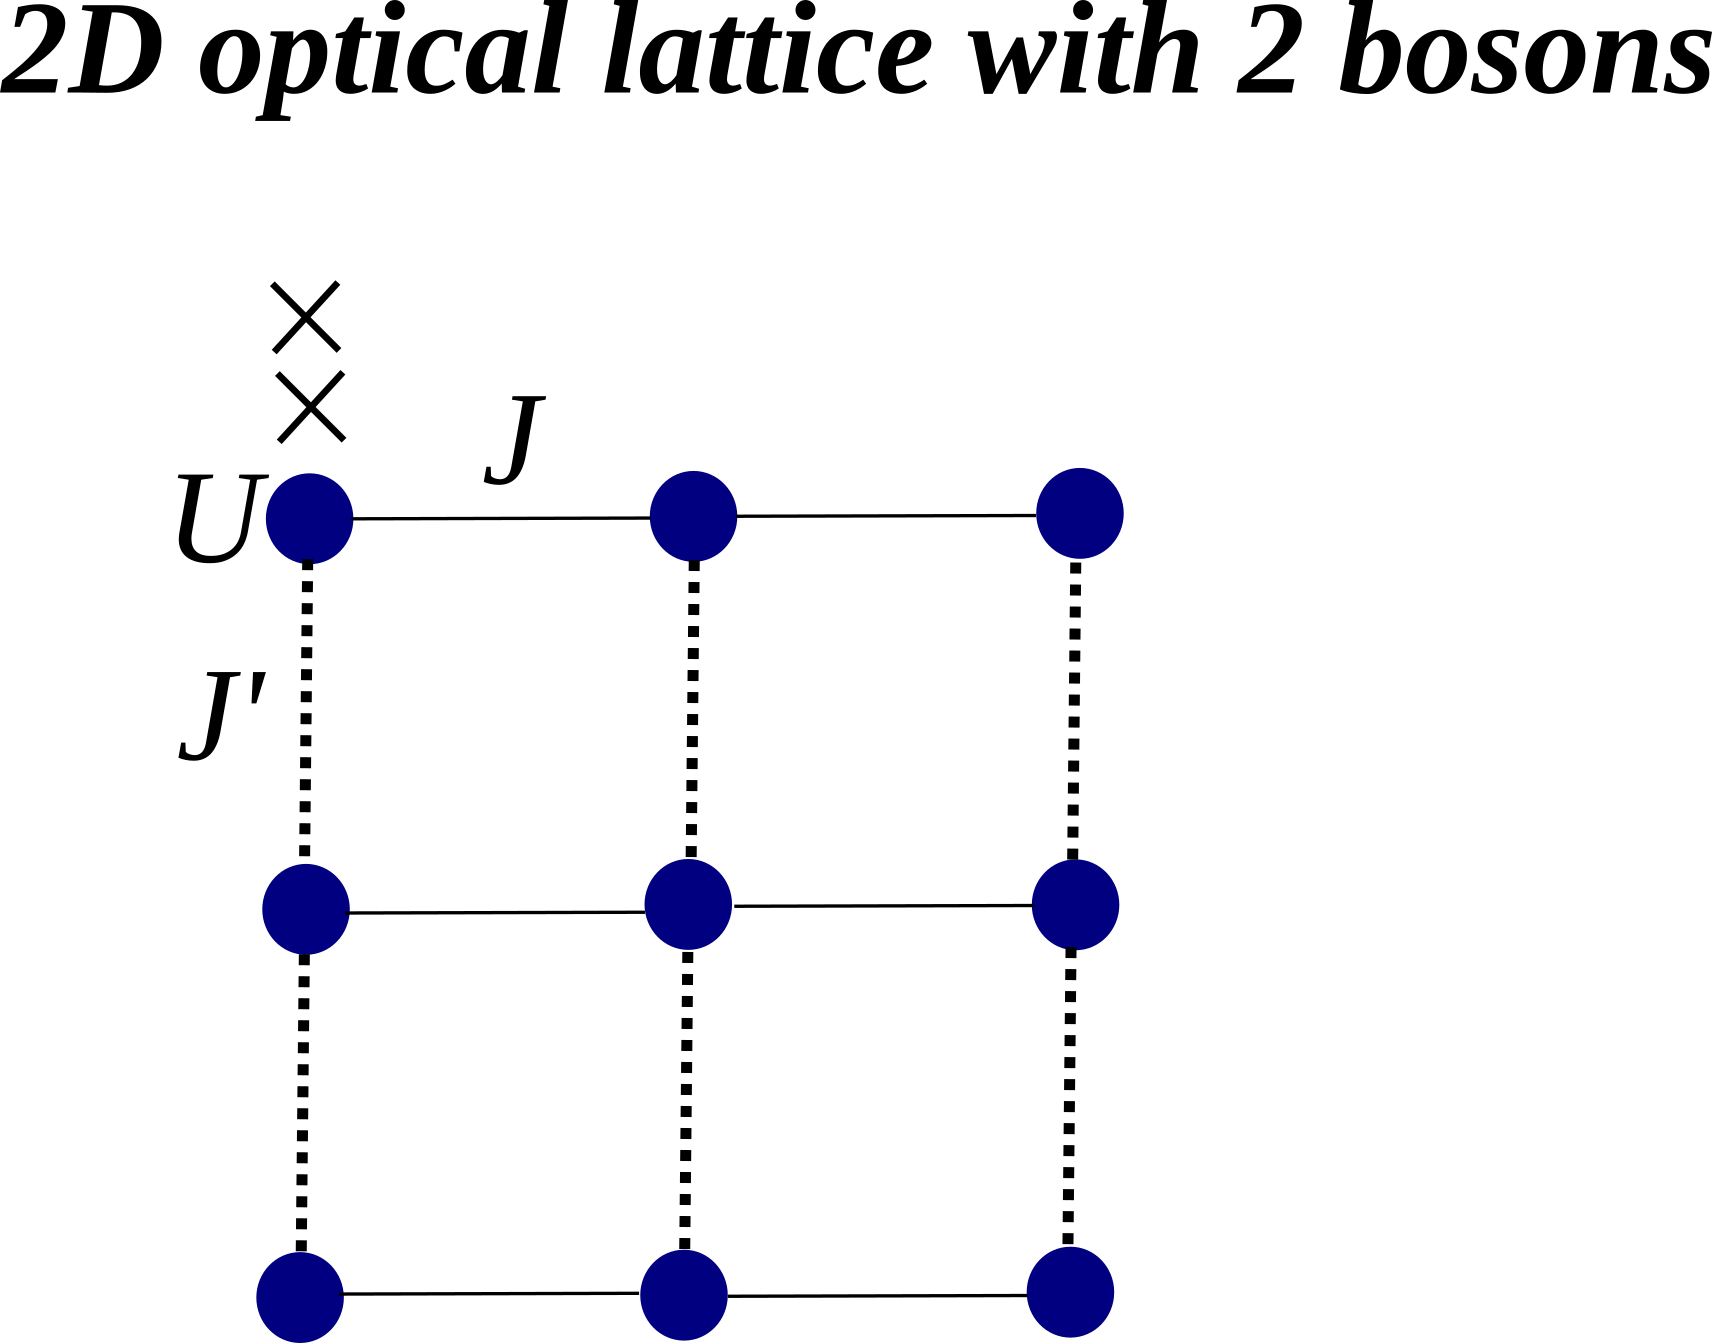
\includegraphics[width=8cm]{lattice_pic}
 \end{center}
 \caption{The blue circles here represent lattice sites and the crosses denote individual bosons. Hopping between any two neighbouring sites on the same chain is characterised by $J$, whereas hopping 
 between chains is characterised by $J'$. A three by three lattice is shown here, but the system can be extended to arbitrary size.}
 \end{figure}

 
We are interested in the time evolution of these systems as it relates to their thermal behaviour.

\newpage
\section{Thermalisation}
 \subsection{Overview}
 
Thermalisation refers to a relaxation of a system to states where the values of macroscopic quantities are stationary, universal with respect to 
widely differing initial conditions, and predictable using statistical mechanics \cite{Rigol2008}. We observe thermalisation in a wide variety of classical systems, and there 
are strong theoretical reasons for anticipating this thermalisation. However, many of these reasons don't apply when considering quantum systems. The question of 
which, if any, quantum systems exhibit thermalisation and how the thermal states can be characterised is of considerable theoretical and experimental interest. 

 \subsection{Classical systems}
To see why thermalisation is common and even expected in many classical systems, we need to understand the property of ergodicity and the impact of chaotic dynamics on it. 
If you start an isolated system in a particular configuration corresponding to a particular point in phase space, it can move through that phase space along the constant-energy
manifold. A system is ergodic if the long-term time average of any single phase space trajectory is equivalent to an ensemble average. \todo{get Kinoshita's definition of ergodicity} 
\todo{Do I need to elaborate on this further?}Classical systems \todo{often? usually? sometimes?} exhibit chaotic dynamics, which are strongly nonlinear and allow the system to quickly 
and essentially uniformly explore the constant-energy manifold irrespective of the initial conditions. This promotes ergodicity, which is implicit in the fundamental assumption of 
statistical mechanics - all accessible microstates are equiprobable. \todo{Need to explicitly link ergodicity and thermalisation, otherwise this is just free-floating and its
relevance is not obvious. What is this link?} This is what leads us to expect our classical systems to thermalise.

 \subsection{Quantum systems}
Quantum systems do not \todo{usually?} exhibit dynamic chaos \todo{see square brackets} [Rigol's line is ``dynamical chaos itself cannot occur in an isolated quantum system, in which the time 
evolution is linear and the spectrum is discrete'' How does that argument work?], so it is not obvious how one would justify applying the assumption of ergodicity in these systems. Because of 
this, it is unclear if, or when, we should expect quantum systems to thermalise, or what statistical ensemble we could use to characterise the relaxed states. 


\section{Integrable systems}
There are a number of classical, isolated systems that do not display thermalisation. The main difference between these systems and those which approach thermal equilibrium is the extent to which
they are constrained relative to the number of degrees of freedom that they posess. This observation is formalised in the notion of integrability. A system is said to be integrable if it has \todo{half? according to 
handout this seems to be the case} as 
many independent integrals of motion (which are conserved) as it has degrees of freedom. An integral of motion for a Hamiltonian is a smooth function $I$ defined on an open subset of the 
phase space such that $\dot{I}=0$ on solutions. \todo{reference handout Danny gave me, I can't see anywhere where its from}So $I(x(t))=\text{constant}$, where $x(t)$ is the solution of the equations of motion
for a particular initial condition. If $x_1(t)$ and $x_2(t)$ are solutions for different initial conditions, then in most cases $I(x_1(t))\ne I(x_2(t))$.
Integrability is a useful property, though it is quite rare. \\\\

Theoretically, we can find exact solutions for the equations of motion for a system if it is integrable, otherwise we cannot. 
In classical mechanics, the idea of integrability is well-understood and neatly defined. The situation in quantum mechanics is much more challenging. One reason for this is that 
the Heisenberg uncertainty principle prevents us from applying the idea of points in phase space with particular trajectories. 
\\\\
With respect to the systems that we are dealing with, it has been shown that a one-dimensional lattice chain of non-interacting bosons is an integrable system \cite{Rigol2007}. 



\todo{see square brackets} [Maybe fall back on ``All 1D systems with conserved energy are integrable'' for U!=0, referencing page 6 of the handout Danny gave me. I don't really know where 
to go for 2D at this point.]

\newpage
\section{Experimental studies}
\subsection{A quantum Newton's cradle}
Kinoshita et. al. investigated \cite{Kinoshita2006} the thermalisation of an out-of-equilibrium 1D Bose gas, which is a  nearly-integrable system. They started with
several thousand arrays of one-dimensional Bose gases, each containing from $40$ to $250$ $^{87}$Rb atoms. The atoms were trapped by combining a blue-detuned \todo{check I understand why this one is 
blue-detuned and the other red-detuned} two dimensional optical lattice, which provides tight transverse confinement, with a red-detuned crossed dipole trap \todo{what is a crossed dipole trap?} 
providing weak axial trapping. In order to create the non-equilibrium momentum distributions, they then pulsed on a $3.2$ THz detuned 1D lattice, which depletesd the zero momentum state
and put the atoms in a superposition momentum state of $\pm2\hbar k$. The two parts of the wavefunction then oscillated out of phase with each other, colliding with each other twice every full cycle
and either reflecting off each other elastically or transmitting straight through like a ``ghostly'' Newton's cradle (see diagram below)

\begin{figure}[H]
 \begin{center}
 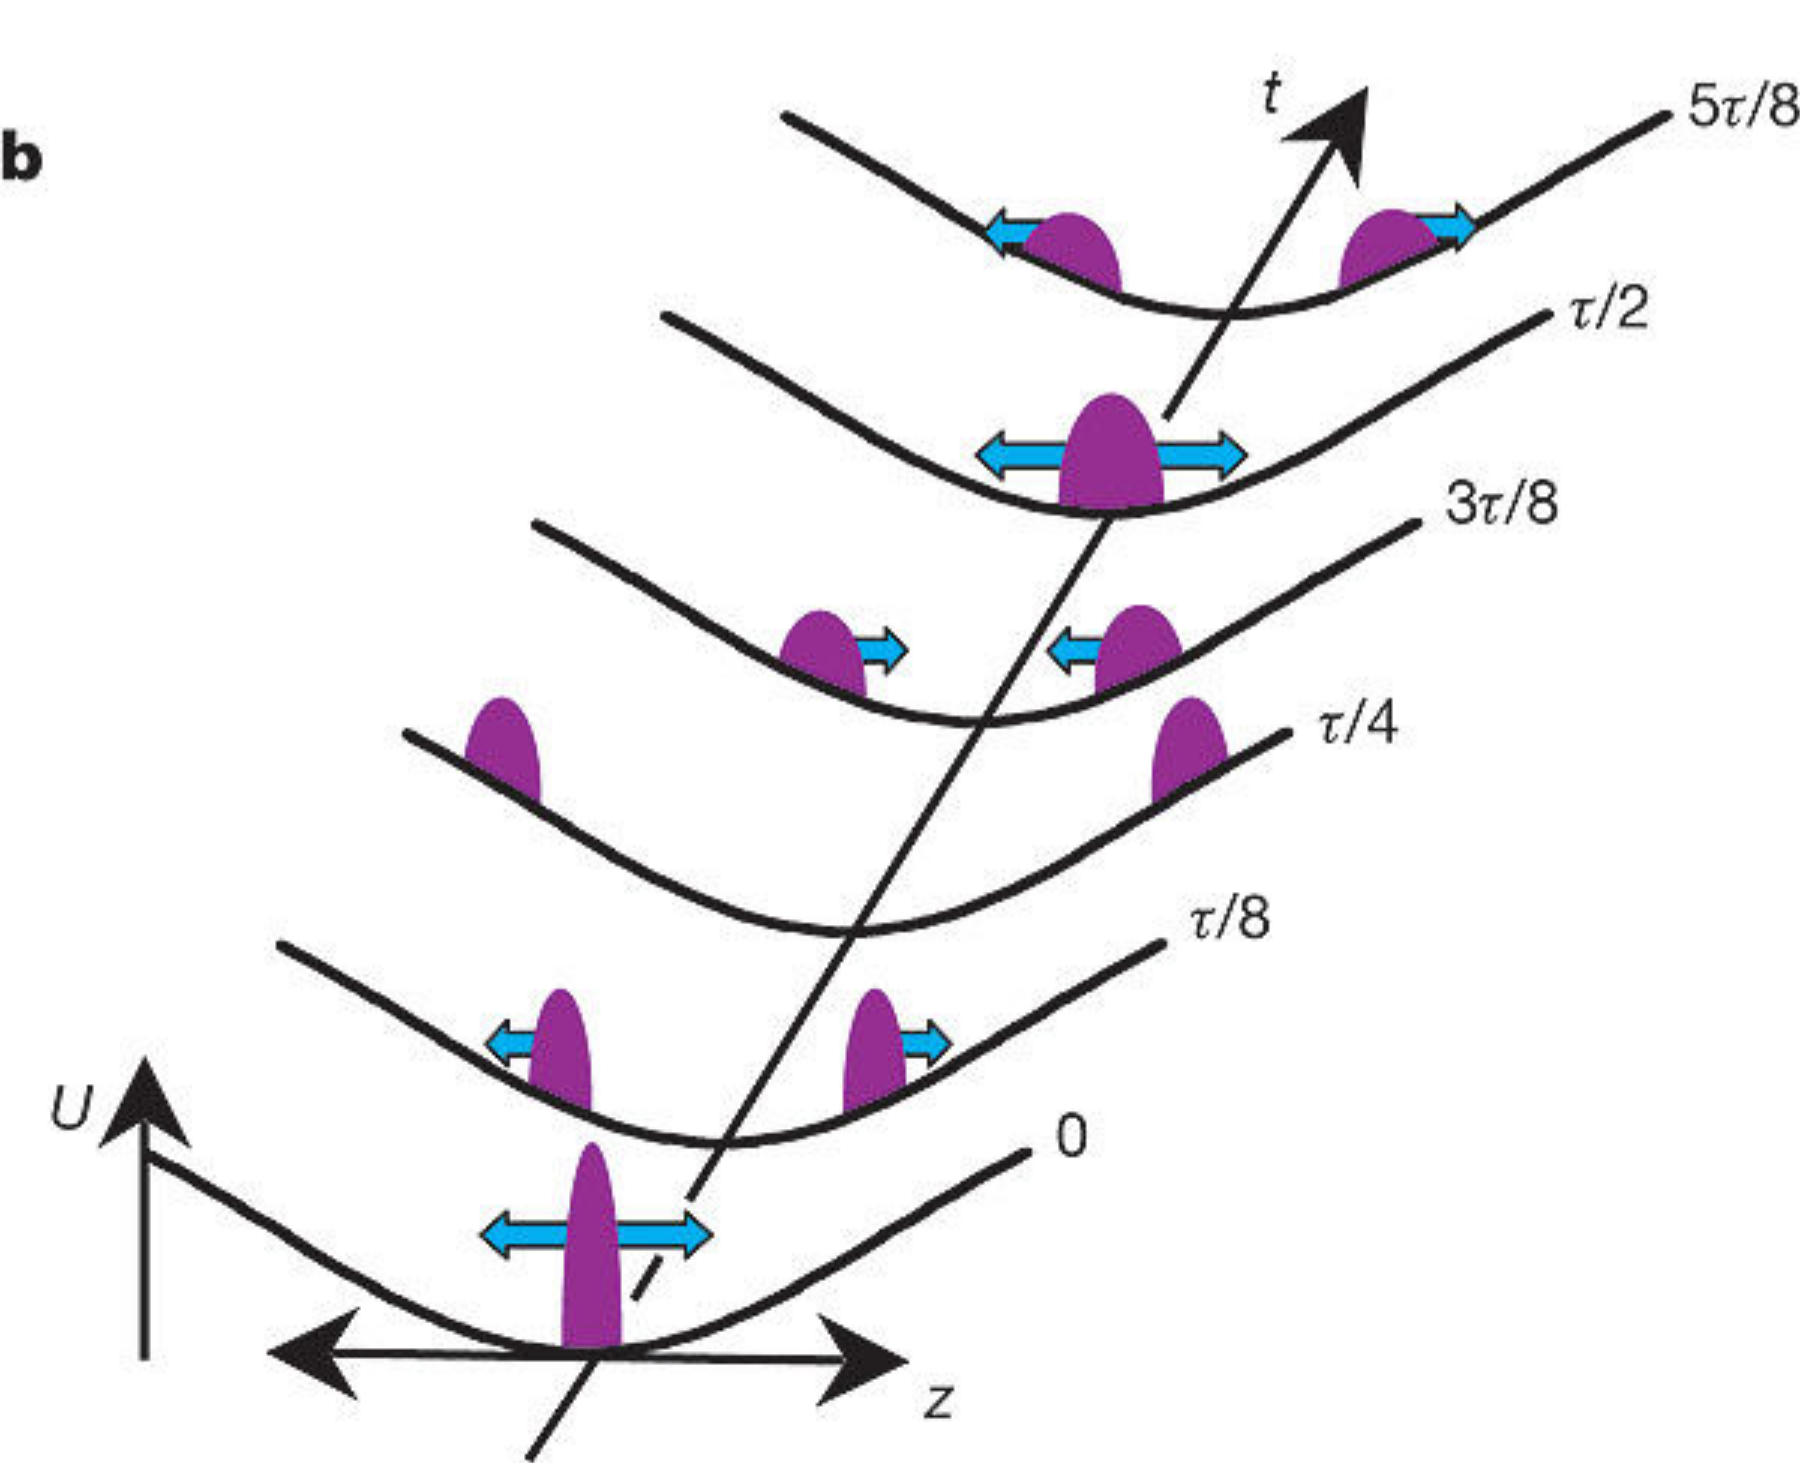
\includegraphics[width=8cm]{quantum_newtons_cradle}
 \end{center}
 \caption{Sketches at various times of two out of equilibrium
clouds of atoms in a 1D anharmonic trap. At time $t=0$ the atoms are put into a momentum superposition with $2\hbar k$ to the right and $2\hbar k$ to the left. The two parts of the 
wavefunction oscillate out of phase with each other with a period $\tau$. Each atom collides with the opposite momentum group
twice every full cycle, for instance, at $t=0$ and $t=\frac{\tau}{2}$. Figure is from reference \cite{Kinoshita2006}.}
 \end{figure}
 
The weak anharmonicity of the trap caused the atoms to gradually dephase. However, the momentum distribution after dephasing was not gaussian (as one would expect for a thermalised state),
and this momentum did not noticeably tend toward this equilibrium distribution, even after thousands of collisions.

\begin{figure}[H]
 \begin{center}
 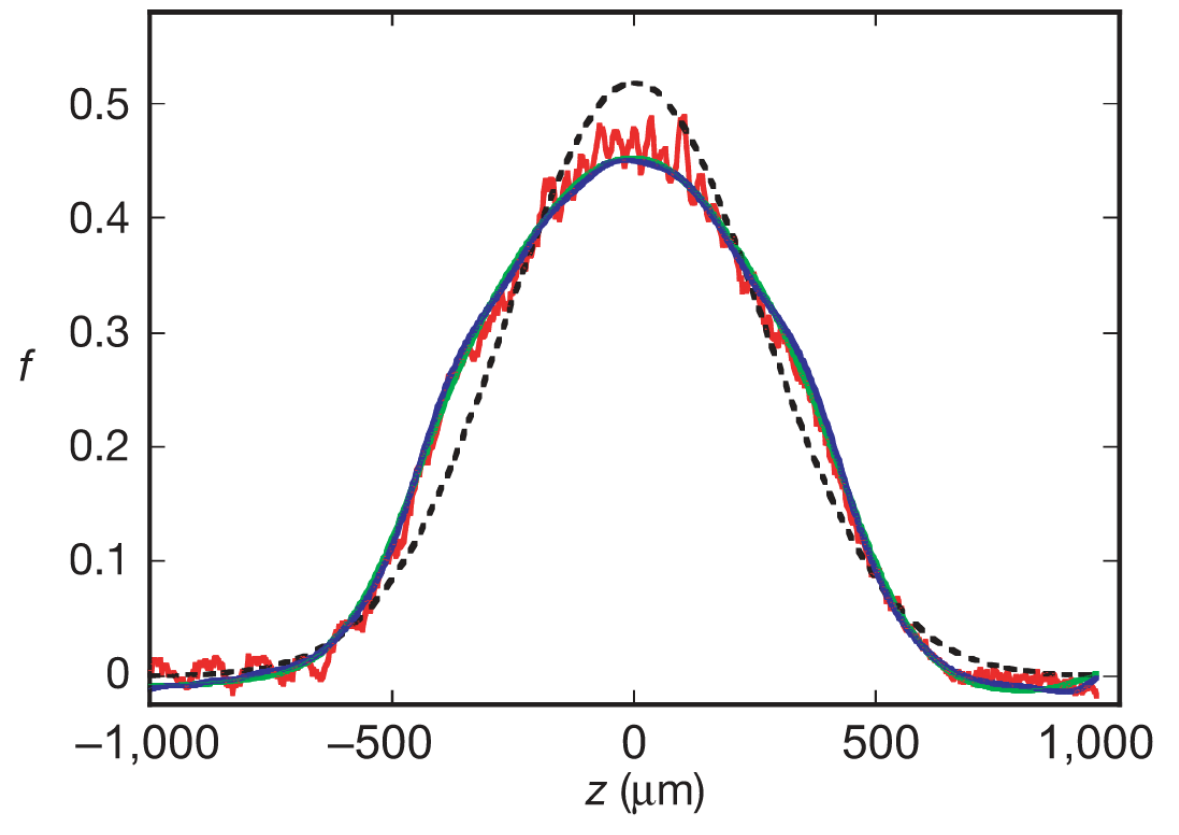
\includegraphics[width=1.0\textwidth]{dephased_momentum_distribution}
 \end{center}
 \caption{\label{dephased_momentum_distribution}The blue and green curves in the above figure are projections from models that take into account loss and heating. The red line is the actual distribution observed. The dashed line 
 is a gaussian with the same number of atoms and r.m.s. width as the actual distribution. }
 \end{figure}
 

To the extent that the actual distribution in figure \ref{dephased_momentum_distribution} conforms to the projected distribution rather than to the gaussian, the atoms have not
thermalized.

These observations extended from the Tonks–Girardeau regime, which has very strong repulsive interactions between bosons so only pairwise collisions can occur, to the intermediate 
coupling regime, where there can be three- (or more) body collisions. 
\newpage
\subsection{Relaxation in a Completely Integrable Many-Body Quantum System}

Inspired by the ``A Quantum Newton's Cradle'' study, investigations were made into a completely integrable many-body quantum system. In this experiment, hard-core bosons \todo{find a good
description of what makes bosons "hard core``} on a 1D lattice were used. The authors, Rigol et. al \cite{Rigol2007}, started with a one dimensional bosonic Hamiltonian with no interactions
and periodic boundary conditions for a lattice with $L$ lattice sites.
\begin{equation}
 \hat{H}=-J\sum_{i=1}^{L} (\hat{a}_{i}^{\dagger}\hat{a}_{i+1}+h.c.)
\end{equation}

They then mapped their bosonic system to a free ferminonic one using a Jordan-Wigner transformation:
\begin{equation}
 \hat{H}=-J\sum_{i=1}^{L} (\hat{c}_{i}^{\dagger}\hat{c}_{i+1}+h.c.)
\end{equation}
Here $\hat{c}_{i}^{\dagger}$ and $\hat{c}_{i+1}$ are fermionic creation and annihilation operators.
The integrals of motion were the fermionic quasi-momentum distribution operators, and the system thus must be integrable because 
there are as many of these operators as they had lattice sites. They have numerically investigated the time evolution of this system and found it to undergo relaxation to an equilibrium 
state. The properties of the state that the system relaxed to were not given by the grand-canonical ensemble, but rather by a generalised Gibbs ensemble, in which the partition function 
is extended to include all of the integrals of motion. 


\begin{figure}[H]
 \begin{center}
 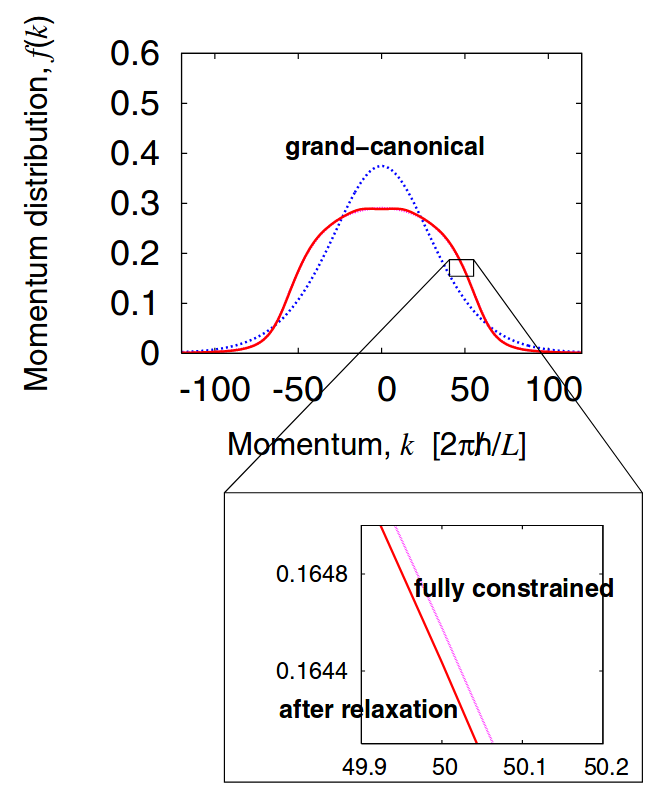
\includegraphics[width=8cm]{grand_canonical_vs_GGE}
 \end{center}
 \caption{Equilibrium (quasi-)momentum distribution after relaxation in comparison with the predictions of the grand-canonical and of
the fully constrained thermodynamical ensembles. The prediction  of the fully constrained  ensemble  is virtually  indistinct
from the results of the dynamical simulation. Image taken from \cite{Rigol2007}.}
 \end{figure}
\todo{the above caption (except the first sentence) is currently copy-pasted from the paper. I'm not sure how to reword those sentences any other way}


They further showed that their generalized equilibrium state carries more memory of the initial conditions than the usual thermodynamic one.

\begin{figure}[H]
 \begin{center}
 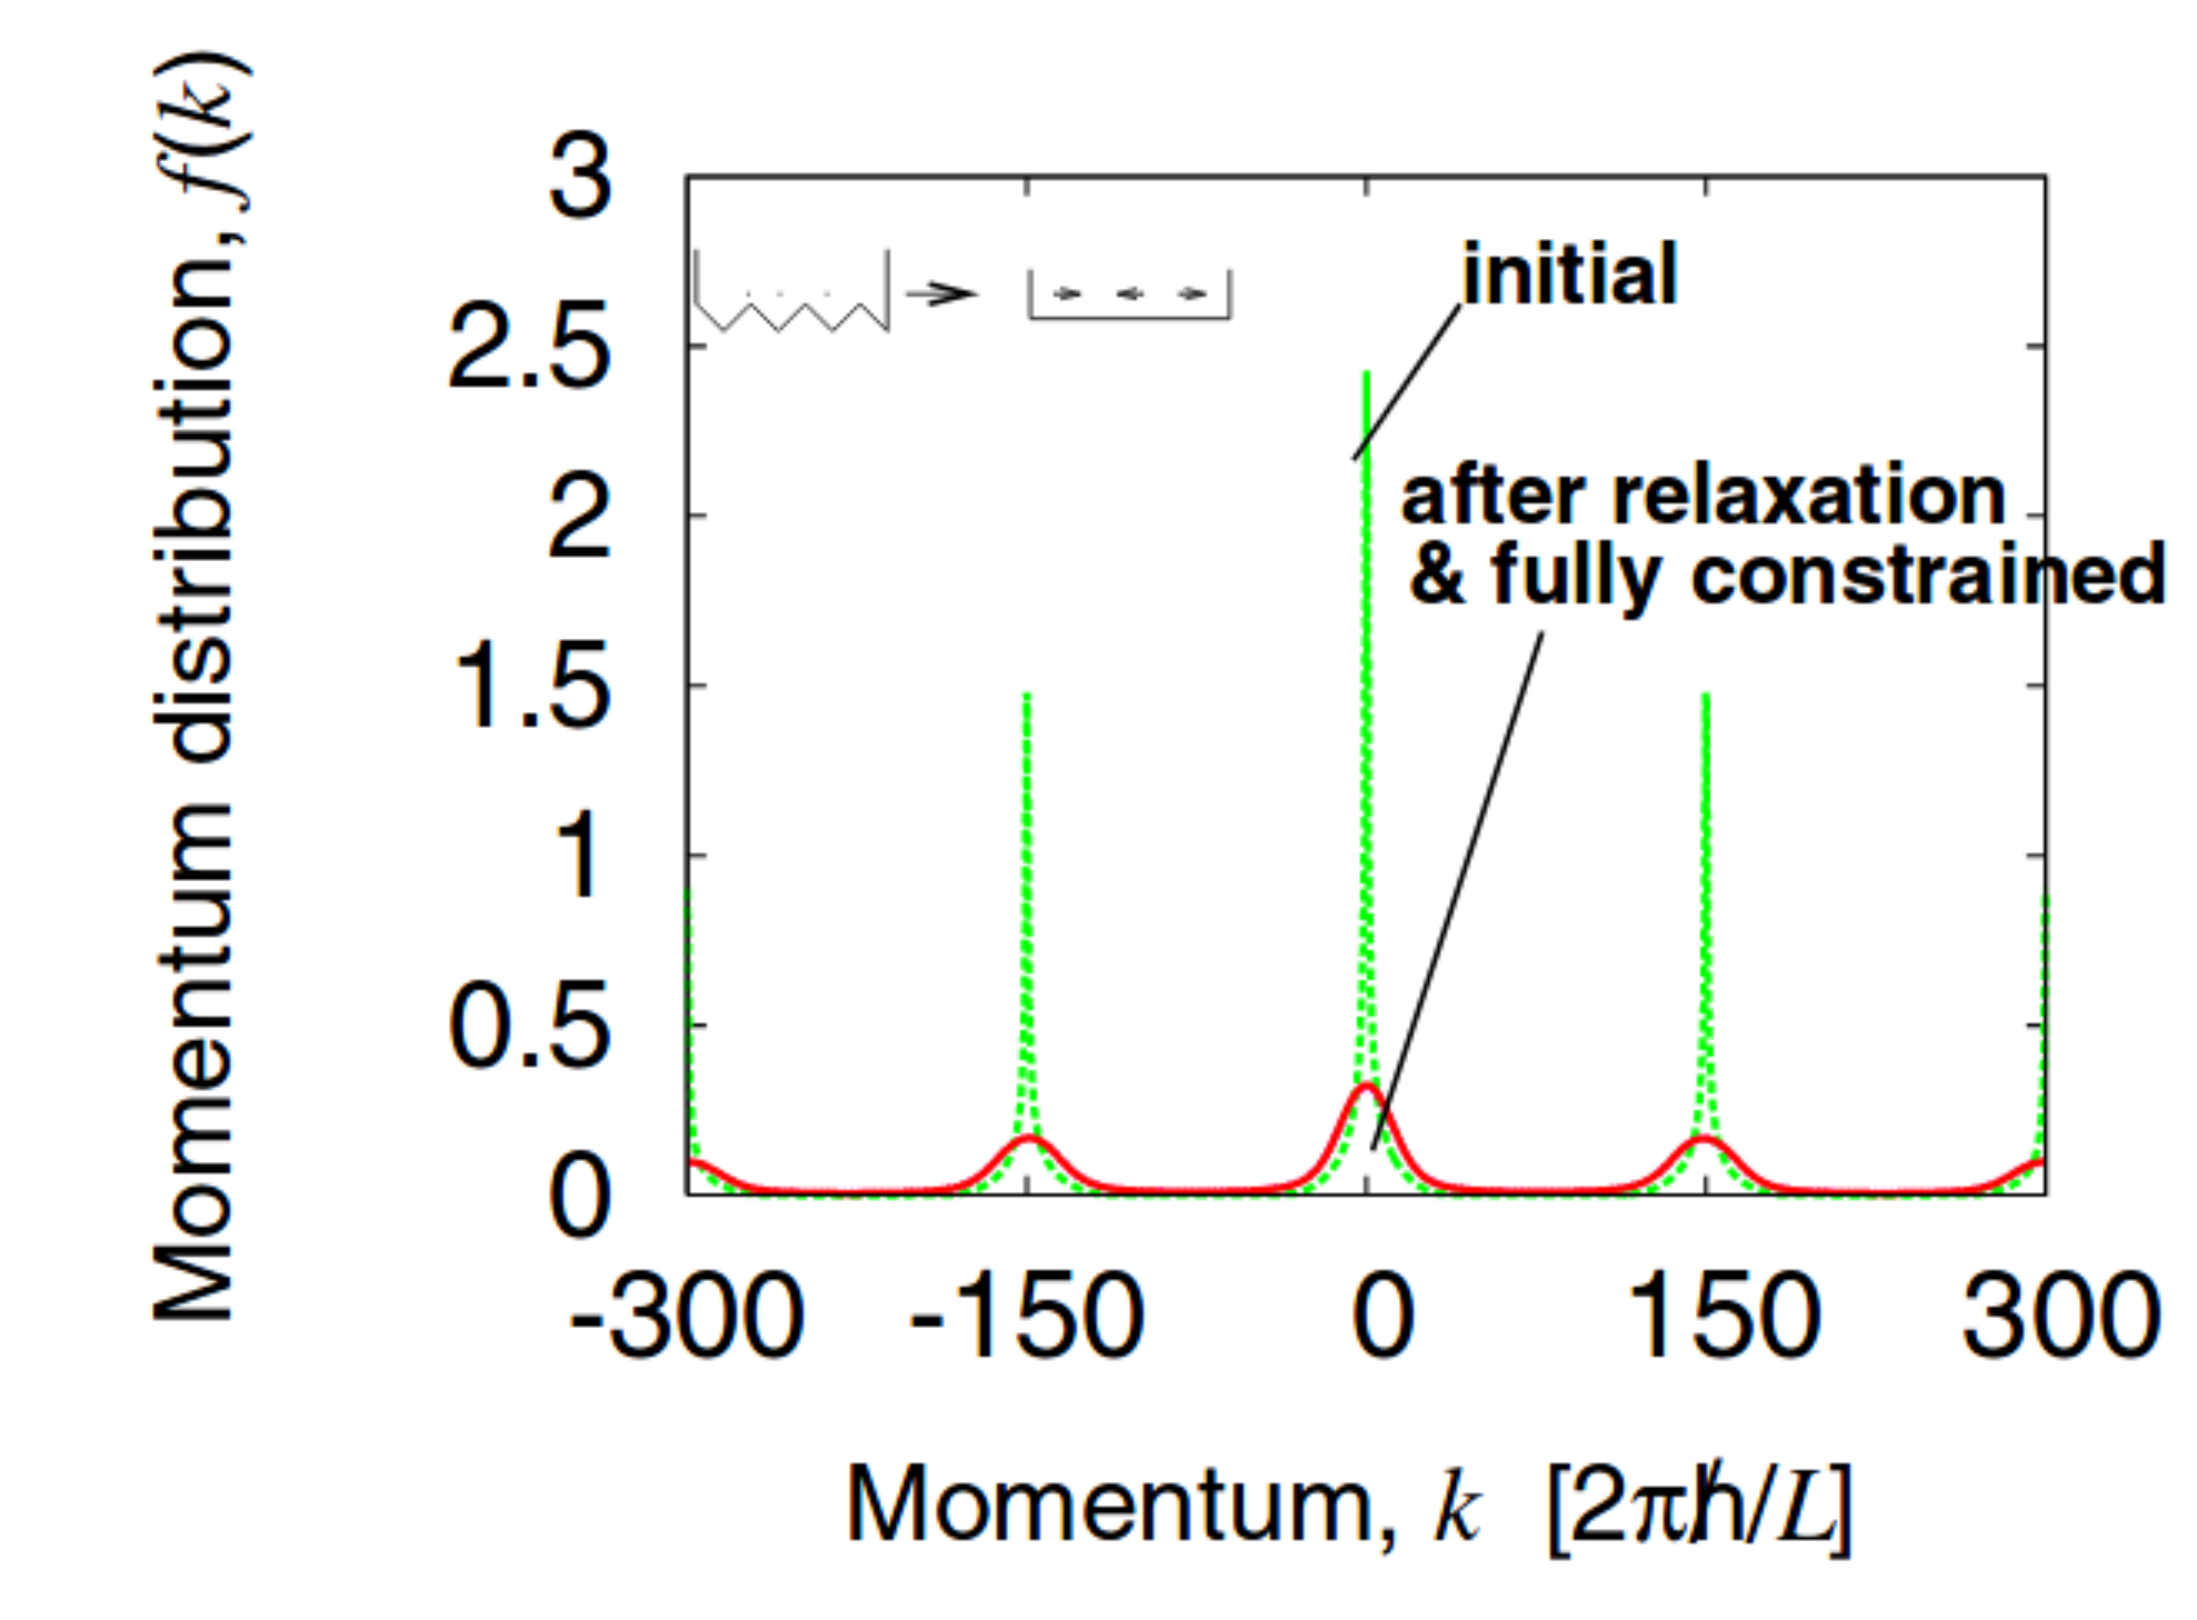
\includegraphics[width=8cm]{after_relaxation_rigol}
 \end{center}
 \caption{The actual quasi-momentum distribution after relaxation vs predictions of the generalised Gibbs ensemble and the grand canonical ensemble. Image taken from \cite{Rigol2007}.}
 \end{figure}

The momentum peaks remain clear and distinct during the whole duration  of  propagation; $t_{\text{fin}}=3000\hbar/J$.

\subsection{Measuring entanglement entropy in a quantum many-body system}
- I still don't see how this is supposed to relate to what I'm doing.
I can write down the definition of the nth order R\'enyi entropies, and describe what purity is. 
I imagine that I could construct a system that is a 2 by N lattice and split it into two one-dimensional lattices of length N, then evaluate their purity (which must be zero for one of the 
chains and 1 for the other if I'm starting with all bosons on one site, right?), then do some second order renyi entropy calculation based on that. Then I could evolve the system in time
and note that this entropy changes. How does that relate the thermalisation? What can I find out from this approach that I don't already get from just looking at expectation values of number 
operators?

\newpage
\section{Results}
\section{Revival}
In a subset of the integrable systems considered, we observed regular instances in which the system would return to the state in which it was initially prepared (it ``revives''). 
To see why we might expect to see revival in some cases, consider the initial state of the system $\ket{\psi(0)}$, which evolves in time according to
\begin{equation}
 \ket{\psi(t)}=e^{i\hat{H}t}\ket{\psi(0)}.
\end{equation}
Now noting that we can use the completeness relation for the energy eigenstates to expand the initial state in the energy basis,
and incorporating the $\hbar^{-1}$ into the time scale,
\begin{align}
 \ket{\psi(t)} =&       e^{i\hat{H}t}\sum_j\ket{E_j}\braket{E_j|\psi(0)}  \nonumber \\
               =&\sum_je^{i\hat{H}t}\ket{E_j}\braket{E_j|\psi(0)} \nonumber \\
                =&\sum_je^{iE_{j}t}\ket{E_j}\braket{E_j|\psi(0)}  \nonumber \\
                =&\sum_j c_{j}e^{iE_{j}t}\ket{E_j}
\end{align}

From here it can be seen that the only time dependence appears in the complex exponentials, each of which is $2\pi$-periodic. If we can find some common time $t_r$ such 
that $E_{j} t_{r}=2 \pi k_{j}$, where $k_{j} \in \mathbb{Z} $ for all $j$, we will recover the initial state exactly, i.e., $\ket{\psi(t_{r})}=\ket{\psi(0)}$. 
The next section describes the conditions necessary for the existence of the revival time.\\
\newpage
\subsection{Exact revival}

We observe an exact and regular revival in precisely the cases in which the eigenvalues are mutually rational, i.e. they are either all rational, or are all rational when 
divided by the same irrational number.
For example, the set of hypothetical eigenvalues $\{0,\sqrt{2},2\sqrt{2},\frac{3\sqrt{2}}{10}\}$ is mutually rational, whereas $\{0,\sqrt{2},\sqrt{3}\}$ is not. In the case of mutually rational eigenvalues, we can write
${E_j}=\frac{p_j}{q_j}$, where $p_j,q_j \in \mathbb{Z}$. The revival time is then given by $t_r=2\pi Q_{LCM}$, where $Q_{LCM}$ is the lowest common multiple of ${q_j}$. 
\\\\
We are yet to find any systems with nonzero interparticle interaction that have mutually rational eigenvalues.
In one dimension, the only systems that we have found that meet the criterion of mutually irrational eigenvalues are those with fewer than 4 lattice sites. In two
dimensions, \todo{do a comprehensive batch of simulations to determine what is and isn't ok in 2D}.

To demonstrate this exact revival, consider a one dimensional lattice with three sites with a single boson and hopping constant $J$ \todo{will go through this section with full generality, not
hard coded numbers soon}. The Hamiltonian for this system is

\begin{equation}
\hat{H}= \begin{bmatrix}
 0 & -J & 0 \\
 -J & 0 & -J\\
 0 & -J & 0
 \end{bmatrix}.
\end{equation}
Diagonalising this matrix yields the eigenvalues $\{-\sqrt{2}J,0,\sqrt{2}J\}$. These are mutually rational (if we divide them all by $\sqrt{2}J$ they are all rational). 
If we rescale the energies by $\sqrt{2}J$ by absorbing that factor into the time scale, then we get eigenvalues $\{-1,0,1\}$.
We can see from the graph of the simulation below that this matches up with a return to the initial state at times that are multiples of $2\pi$.
%\todo{use data from '3by1_revival_data' folder to get this to plot properly once you ask Danny how to put fractions in axis titles}

\begin{figure}[H]
 \begin{center}
 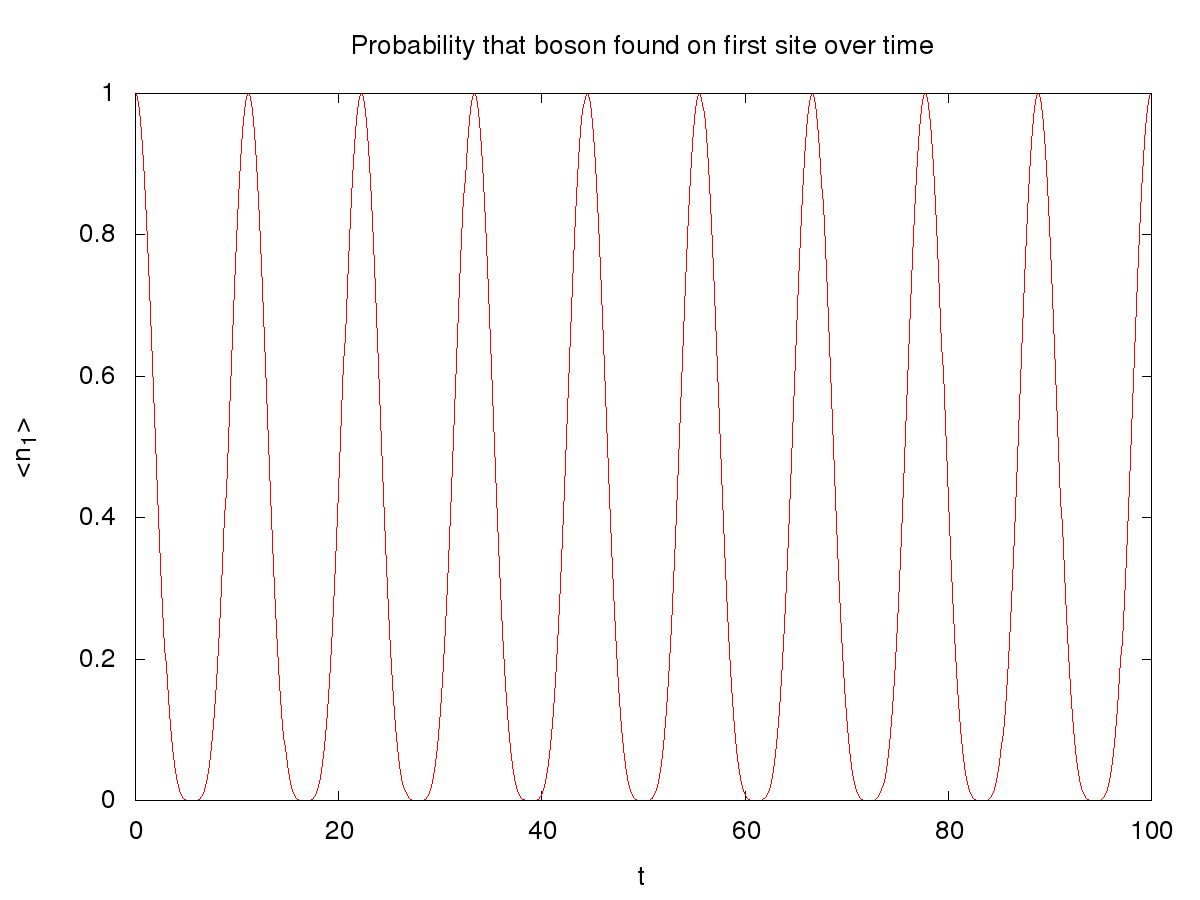
\includegraphics[width=1.0\textwidth]{showing_revival_3by1}
 \end{center}
\end{figure}

The reason that there appear to be several revivals that our method ``misses'' is that states with different phases in the coefficients of the eigenvectors can also produce $\langle n_1 \rangle =1$, whereas the revival time that is 
calculated in our method corresponds to exact revival of the initial wavefunction.

\subsection{Approximate revival}
The range of systems for which the spectrum \todo{is it inaccurate to describle the spectrum (as opposed to the eigenvalues) as mutually irrational?} is mutually rational is a small one. 
All systems which have nonzero interparticle interactions have mutually irrational eigenvalues. One of the most interesting results so far is that even in the one dimensional single particle case,
if there are more than three lattice sites, the spectrum will be irrational. We can demonstrate this by considering a single chain of five sites with one boson. The Hamiltonian for this 
system is \\\\
\begin{equation}
\hat{H}= \begin{bmatrix}
 0 & -J & 0 & 0 & 0\\
 -J & 0 & -J & 0 & 0\\
 0 & -J & 0 & -J & 0\\
 0 & 0 & -J & 0 & -J\\
 0 & 0 & 0 & -J & 0
 \end{bmatrix}.
\end{equation}
\\\\
The eigenvalues of this system are $\{-\sqrt{3}J,-J,0,J,\sqrt{3}J\}$. These are clearly not mutually rational, so we cannot find an exact revival time for this system, despite the fact that it is 
fully integrable. Running a simulation of this system where we start the boson off on the first site, we find that the probability of finding the boson on the first site never quite reaches $1$ again.

\todo{run this again with the xaxis labelled 't/J'}
\begin{figure}[H]
 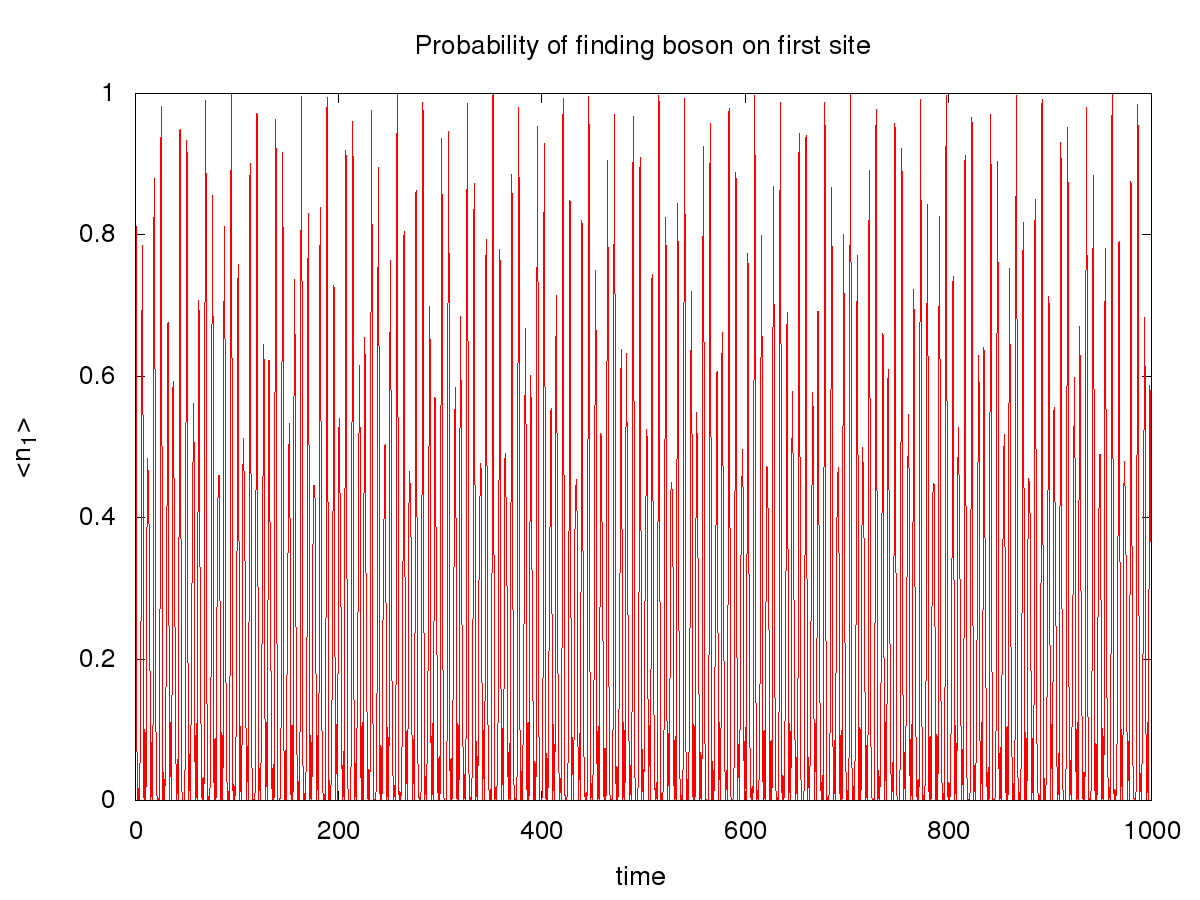
\includegraphics[width=1.0\textwidth]{5_by_1_T1e4_U0}
 \centering
\end{figure}

Judging the figure above by eye, it may appear that we have exact revival, but this is not actually the case. If we look at how long it takes for the system to get within epsilon of
its initial state (i.e. $||\ket{\psi(t)}-\ket{\psi(0)}||<\epsilon$)
we get the graph below. Note that $t^*$ denotes the time at which the system got within a particular value of $\epsilon$ of the initial state.
\begin{figure}[H]
 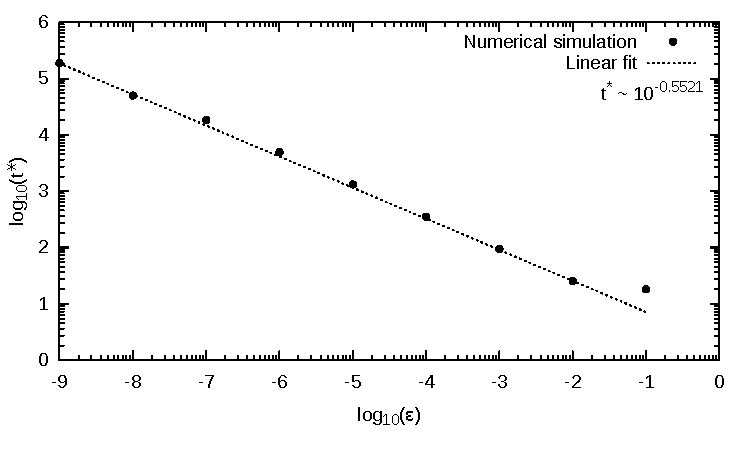
\includegraphics[width=1.0\textwidth]{recurrence_times}
 \centering
\end{figure}
While we see that the system does appear to get arbitrarily close to revival, but it can take arbitrarily long to do so. This result can be explained in terms of the Poincar\'e recurrence theorem.
\newpage
\section{The Poincar\'e Recurrence Theorem}

In 1890, Henri Poincar\'e proved the following theorem for classical mechanics: "Any phase-space configuration $(q,p)$ of a system enclosed in a finite volume will be repeated as accurately as one wishes
after a finite(be it possibly very long) interval of time'. This theorem was extended to quantum systems in 1956 by P. Bocchieri and A. Loinger\cite{Bocchieri1957}, where it takes a slightly different
form:"Let us consider a system with discrete energy eigenvalues $E_n$; if $\psi(t_0)$ is its state vector in the Schr{\"o}dinger picture at the time $t_0$ and $\epsilon$ is any positive number, at 
least one time T will exist such that the norm $||\ket{\psi(T)}-\ket{\psi(t_0)}||$ of the vector $\ket{\psi(T)}-\ket{\psi(t_{0})}$ is smaller than $\epsilon$."

\subsection{Proof}
The proof presented by Bocchieri and Loinger shows the theorem to be true for an infinite-dimensional system. In this dissertation, we investigate only finite-dimensional systems, and a simpler version of 
the proof can be constructed. Let $D$ be the dimensionality of the system (an expression for calculating $D$ will be derived later \todo{See square brackets}[Should I do this later? Or make a section earlier? Where should it go?]).
We will first show that there exists a time $T$ at which $||\ket{\psi(T)}-\ket{\psi(t_0)}||^2<\epsilon'$ for any $\epsilon'>0$ and then extend this to $||\ket{\psi(T)}-\ket{\psi(t_0)}||<\epsilon$. Note that in
the following we will introduce the notation $\tau=T-t_0$ and $\alpha^2=||\ket{\psi(T)}-\ket{\psi(t_0)}||^2$.

\begin{align*}
 \alpha^2=&\left(\bra {\psi(T)}-\bra {\psi(t_0)}\right)\left(\ket{\psi(T)}-\ket{\psi(t_0)}\right) \\
 = \ &2-\braket{\psi(T)|\psi(t_0)}-\braket{\psi(t_0)|\psi(T)} \\
 = \ &2-\left(\sum_{n=1}^{D}c_n^* e^{iE_{n}T}\bra{E_n}\right)\left(\sum_{j=1}^{D}c_je^{-iE_{j}t_{0}}\bra{E_j}\right)-\left(\sum_{j=1}^{D}c_j^*e^{iE_{j}t_{0}}\ket{E_j}\right)\left(\sum_{n=1}^{D}c_n e^{-iE_{n}T}\ket{E_n}\right) \\
 = \ &2-\left(\sum_{n=1}^D |c_n|^2 e^{iE_{n}(T-t_0)}+\sum_{n=1}^D |c_n|^2 e^{-iE_{n}(T-t_0)}\right) \ \ \ \text{since} \braket{E_j|E_n}=\delta_{ij} \\
 = \ &2\left(\sum_{n=1}^D |c_n|^2\left(1-cos\left(E_{n}\tau\right) \right) \right) \ \ \text{because}  \ \sum_{n=1}^D |c_n|^2=1 \\
 \leq\ &2\left(\sum_{n=1}^D\left(1-cos\left(E_{n}\tau\right) \right) \right)
\end{align}
\todo{is that last inequality valid?}
It is sufficient to show that there exists a value of $\tau$ such that $\sum_{n=1}^D\left(1-cos\left(E_{n}\tau\right) \right)<\hat{\epsilon}$. \todo{I've gotten myself into some messy 
notation here with 3 different defined epsilons.} This is actually the case according to a standard result of the theory of the almost-periodic functions.\todo{need reference! The one from Bocchieri is in German.}
\\\\
From here I can show that if $||\ket{\psi(T)}-\ket{\psi(t_0)}||^2<\epsilon'$ then $||\ket{\psi(T)}-\ket{\psi(t_0)}||<\sqrt{\epsilon'}$ and define $\epsilon=\sqrt{\epsilon'}$. I also have to define $\epsilon'=2\hat{\epsilon}$.
However, I'd rather not write this out before making the notation cleaner.

\newpage
\bibliographystyle{plain}
\bibliography{honours}


%Note: \url{https://arxiv.org/pdf/1007.5331.pdf} has a good description of what quantum ergodicity is on page 10
%\\ Note: \url{http://www.physicspages.com/tag/field-operators/} was the thing that made field operators make some sense for me
%\\Note: \url{http://www.nucleares.unam.mx/~alberto/apuntes/altland.pdf} was super useful for background second quantisation.
%\\Note: \url{http://iopscience.iop.org/article/10.1209/epl/i2004-10265-7/pdf} mentions finding the 1D B-H model to not be integrable. This could be v useful when including U(n*n-n) term
%\\Note: \url{https://arxiv.org/pdf/cond-mat/0410614v1.pdf} might have good stuff for background section of dissertation
%\newpage


%\section{Additional questions for Danny}




\end{document}